\documentclass[main.tex]{subfiles}
\begin{document}

\chapter{Stein Variational Gradient Descent}
En la sección \ref{sec:advi} introdujimos la idea de hacer inferencia variacional a través de transformaciones suaves. El algoritmo \eqref{algo:advi} le quita restrucciones al problema variacional completando el soporte $\X\subseteq\RR^d$ de la densidad de interés a $\RR^d$ completo y después minimiza $\kl$ con familias de normales, una solución paramétrica. Este proceso utilliza una librería de transformaciones y sus jacobianos que el equipo de desarrollo de la implementación mantiene\cite{advi}, pero en principio no se necesita salir de $\X$. La idea detrás de SVGD es partir de una distribución $Q_0$ sobre $\X$ y construir de manera iterativa y no paramétrica biyección suave $T: \X \to \X$ que minimice $\kl(T_*Q_0\mmid P)$.

% ------------------------------------------------------------------------------
% ------------------------------------------------------------------------------
% ............................. EL MÉTODO DE STEIN .............................
% ------------------------------------------------------------------------------
% ------------------------------------------------------------------------------
\section{El método de Stein}

El primer ingrediente necesario es un resultado en teoría de probabilidad que Charles Stein publicó en 1972 para dar una cota explícita a la convergencia en distribución del teorema central del límite, pero que tiene aplicación en muchos otros contextos de aproximación \cite{stein-magic-method, formal-stein-method}. En su forma general, el método de Stein involucra dos medidas de probabilidad $P, Q$ en el mismo espacio $\X$; de las cuáles conocemos de forma completa sólo $Q$ y queremos usarla para aproximar $P$, acotando el error. En inferencia variacional $P$ es la distribución posterior y $Q$ queda bajo nuestro control. Algunas aplicaciones modernas de corte teórico están documentadas en \url{https://sites.google.com/site/steinsmethod/home}. 


En lo que sigue, $\X$ es un subconjunto de $\RR^d$.

\begin{definition}
    $ \mathcal{H} \subseteq \{h: \X \to \R \textrm{ continua y acotada}\}$ es una \textit{clase (de funciones) separadora} si cuando 
    \begin{equation*}
        \E_Ph = \E_Qh \quad \forall h \in \mathcal{H} 
    \end{equation*}
    se sigue que $P=Q$. Es decir, basta conoer la integral de las funciones en $\mathcal{H}$ con respecto a $P$ y $Q$ para concluir la igualdad como medidas.
\end{definition}

Ignorando por el momento el problema de existencia (que probaremos más adelante), consideremos una clase separadora $\mathcal{H}$. Para cada $h \in \mathcal{H}$, supongamos que puede encontrarse una solución $f_h$ la \textit{ecuación de Stein}

\begin{equation}\label{eq:stein-equation}
    h - \E_Qh = \A f
\end{equation}

y sea $\F = \{f_h: h \in \mathcal{H}\}$. Integrando con respecto a $P$ de ambos lados, obtenemos
\begin{equation}\label{eq:integrated-stein-equation}
    \E_Ph - \E_Qh = \E_P[\A f]
\end{equation}

De la ecuación \eqref{eq:integrated-stein-equation} y por ser $\mathcal{H}$ una clase separadora, se sigue que 
\begin{align*}
    P = Q &\Leftrightarrow \\
    &\Leftrightarrow \E_Ph - \E_Qh = 0 \quad \forall h \in \mathcal{H}  \\
    &\Leftrightarrow \E_P[\A f]= 0 \quad \forall h \in \mathcal{H}
\end{align*}

Así que encontramos condiciones necesarias y suficientes para que $P=Q$ en términos de $\A$ y $\F$. 

\begin{definition}
    La \textit{caracterización de Stein} de $P$ es
    \begin{equation*}
        X\sim P \Leftrightarrow \E_{x\sim P}[\A f(x)]= 0 \quad \forall f \in \F
    \end{equation*}
    donde $\A$ recibe el nombre de \textit{operador de Stein para } P y $\F$ {clas de Stein} de $P$.
\end{definition}

Aterricemos ideas con un ejemplo antes de continuar las generalidades. El siguiente lema es el resultado original de Stein (en su versión para la distribución normál estandar), que encuentra de manera explícita el operador $\A$  y una clase separadora. 

\begin{theorem}[El lema de Stein]
    $Z \sim \mathcal{N}(0, 1)$ si y sólo si 

    \begin{equation*}
        \E\left[Zf(Z)\right] = \E\left[f'(Z)\right]
    \end{equation*}
    
    para toda $f: \RR \to \RR$ absolutamente continua tal que $\E | f' | < \infty$.
    \begin{proof}
        Supongamos primero que $f$ tiene soporte compacto contenido en $(a, b)$, con $a, b \in \overline{\RR}$. Integrando por partes con $u=f(z)$ y $dv = ze^{\frac{-z^2}{2}}$,
        \begin{align}\label{eq:stein-parts}
        \begin{split}
            \E[zf(z)] &= \int_a^b zf(z)e^{\frac{-z^2}{2}}dz \\
                &= \left[f(z)e^{\frac{-z^2}{2}} \right]_a^b 
                    + \int_a^b f'(z)e^{\frac{-z^2}{2}}dz
        \end{split}
        \end{align}
        La hipótesis sobre el dominio hace que el primer término se anule, y el segundo es precisamente $\E[f'(Z)]$. 

        En general $f$ puede tener a todo $\RR$ de dominio, pero en la prueba la \enquote{recortaremos} para utilizar el resultado de arriba. Formalmente, supongamos ahora que $f$ satisface las hipótesis del teorema, y que además tanto $\E[Zf(Z)]$ como $E[f'(Z)]$ son finitas.
        Sea $(g_n)_{n\in\N}$ la sucesión de funciones
        \begin{equation*}
            g_n(z) = 
            \begin{cases}
                0, & z < -2n \\
                \frac{1}{n}(z+2n), & -2n \leq z < -n \\
                1, & -n \leq z \leq n \\
                \frac{-1}{n}(z-2n), & n < z \leq 2n \\
                0, & \quad z > 2n
            \end{cases}
        \end{equation*}
        \begin{figure}
            \centering
            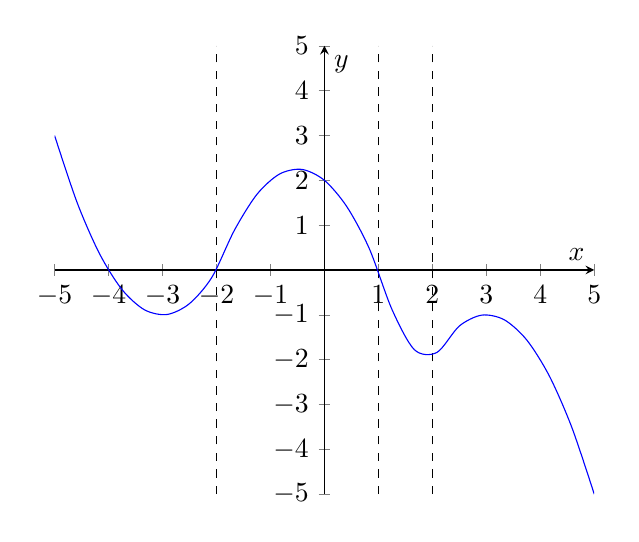
\begin{tikzpicture}[
                declare function={
                func(\x)= (\x<=-2) * (\x*\x + 6*\x + 8)   +
                and(\x>-2, \x<=1) * (2 - \x - \x*\x)     +
                and(\x>1,  \x<=2) * (6 - 8*\x + 2*\x*\x) +
                            (\x>2) * (-10 + 6*\x - \x*\x);
                }
            ]
            \begin{axis}[
                axis x line=middle, axis y line=middle,
                ymin=-5, ymax=5, ytick={-5,...,5}, ylabel=$y$,
                xmin=-5, xmax=5, xtick={-5,...,5}, xlabel=$x$,
            ]
            \pgfplotsinvokeforeach{-2, 1, 2}{
                \draw[dashed] ({rel axis cs: 0,0} -| {axis cs: #1, 0}) -- ({rel axis cs: 0,1} -| {axis cs: #1, 0});}
            \addplot[blue, domain=-5:5, smooth]{func(x)};
            \end{axis}
            \end{tikzpicture} 
            \caption{Se supone que son los trapecios}\label{fig:trapecios}
        \end{figure}
        Es decir, la familia de funciones en la figura \ref{fig:trapecios} \textcolor{red}{(que claramente no es porque se ve que hacer la figura en tix es todo un tema)}. Construimos una segunda sucesión definiendo
        \begin{equation*}
            f_n(z) = f(z)g_n(z)
        \end{equation*}
        Sin importar $n$, $f_n$ es una función con soporte compacto, por lo que aplica la ecuación \eqref{eq:stein-parts}. Además, se cumple para toda $z$ que
        \begin{equation*}
            \mid f_n(z) \mid = | f(Z) | \mid g_n(z) \mid \leq | f(Z) |
        \end{equation*}
        y que $f_n(x) \rightarrow f(x)$ puntualmente. Más aún, también $f_n'(x) \rightarrow f'(x)$ puntualmente, pues
        \begin{equation*}
            g'_n(z) = 
            \begin{cases}
                0, & z < -2n \\
                2 + \frac{z}{n}, & -2n \leq z < -n \\
                0, & -n \leq z \leq n \\
                2 - \frac{z}{n}, & n < z \leq 2n \\
                0, & \quad z > 2n
            \end{cases}
        \end{equation*}
        y después de usar la regla de la cadena y simplificar
        \begin{equation*}
            f'_n(z) = 
            \begin{cases}
                0, & z < -2n \\
                2f'(x), & -2n \leq z < -n \\
                f'(x), & -n \leq z \leq n \\
                2f'(x), & n < z \leq 2n \\
                0, & \quad z > 2n
            \end{cases}
        \end{equation*}
        Así que siempre puede encontrarse $n$ suficientemente grande para que $f'(x) = f'_n(x)$.
        
        Como supusimos integrabilidad de $\mid f \mid$, el teorema de la convergencia dominada asegura que
        \begin{align}
        \begin{split}
            \E[Zf(Z)] &= \int_{-\infty}^\infty zf(z)e^{\frac{-z^2}{2}} dz \\
            &= \lim_{n\rightarrow\infty}\int_{\RR}zf_n(z)e^{\frac{-z^2}{2}} dz \\
            &= \lim_{n\rightarrow\infty}\left(
                    \left[f_n(z)e^{\frac{-z^2}{2}} \right]_{-\infty}^\infty  + \int_{-\infty}^\infty f_n'(z)e^{\frac{-z^2}{2}}dz
                \right) \\
            &= \lim_{n\rightarrow\infty}0 + \lim_{n\rightarrow\infty}\int_{-\infty}^\infty f_n'(z)e^{\frac{-z^2}{2}}dz \\
            &= \int_{-\infty}^\infty f'(z)e^{\frac{-z^2}{2}}dz \\
            &= \E[f'(Z)]
        \end{split}
        \end{align}
        Finalmente, basta notar que por los lemas \eqref{lemma:stein-f1} y \eqref{lemma:stein-f2}, no era necesario aumentar hipótesis. Si $\E[f'(Z)] < \infty$, también se tiene que $\E[| f(Z) |], \E[Zf(Z)] < \infty$.

        Para probar el converso, supongamos que $W$ es una variable aleatoria que satisface $\E\left[Wf(W)\right] = \E\left[f'(W)\right]$. \textcolor{red}{Probar el converso}.
    \end{proof}
\end{theorem}

\begin{lemma}\label{lemma:stein-f1}
    Si $Z\sim \mathcal{N}(0, 1)$ y $f$ es una función absolutamente continua tal que $\E[|f'(Z)|] < \infty$, entonces $\E[| f(Z) |] < \infty$.
    \begin{proof}
        Analicemos casos. Si $z \in [-1, 1]$, 
        \begin{equation*}
            |f(z)| \leq \sup_{|x|\leq 1} |f(x)| \leq \sup_{|x|\leq 1} |f(x)| + |zf(z)|
        \end{equation*}
        En cualquier otro caso, 
        \begin{equation*}
            |f(z)| \leq |z||f(z)| \leq  \sup_{|x|\leq 1} |f(x)| + |zf(z)|
        \end{equation*}
        por lo que la cota es válida para toda $z$. De la continuidad de $f$ y el teorema de Weirestrass se sigue que el supremo sea finito.
    \end{proof}
\end{lemma}

\begin{lemma}\label{lemma:stein-f2}
    Si $Z\sim \mathcal{N}(0, 1)$ y $f$ es una función absolutamente continua tal que $\E[|f'(Z)|] < \infty$, entonces $\E[|Zf(Z)|] < \infty$.
    \begin{proof}
        Sea $\phi$ la densisdad normal estándar.
        \begin{align*}
            \E[|Zf(Z)|] &= \int_{\RR} |zf(z)|\phi(z)dz \\
            &\leq \int_{\RR}|z|\left(\left|f(z)-f(0)\right|+\left|f(0)\right|\right)\phi(z) dz \\
            &= \int_0^\infty z|f(z)-f(0)|\phi(z)dz + \int_{-\infty}^0(-z)|f(0)|\phi(z)dz \\
                &\qquad  + |f(0)|\int_{\RR}\left|z\right|\phi(z)dz
        \end{align*}
        Para acotar el tercer sumando, basta recordar que si $X\sim \mathcal{N}(0, 1)$, entonces $\left|X\right| \sim \text{MediaNormal}(0,1)$, que tiene media $\sqrt{\frac{2}{\pi}}$. Aplicando el teorema fundamental del cálculo a $f$ y la desigualdad $\left|\int g\right|\leq \int\left|g\right|$, podemos acotar el resto de la suma con
        \begin{equation}\label{eq:stproof-cota}
            \int_0^\infty z\int_0^z\left|f'(t)\right|dt\phi(z)dz 
                + \int_{-\infty}^0(-z)\int_z^0\left|f'(t)\right|dt\phi(z)dz
        \end{equation}
        Que gracias al teorema de Fubini, la identidad $\phi'(z) = -z\phi(z)$ y el hecho $\lim_{z\rightarrow \pm\infty}\phi(z) = 0$ puede reescribirse como
        \begin{align*}
            \eqref{eq:stproof-cota} &= \int_0^\infty \left|f'(t)\right|\int_t^\infty z\phi(z)dzdt
                + \int_{-\infty}^0\left|f'(t)\right|\int_{-\infty}^t(-z)\phi(z)dzdt \\
            &= \int_0^\infty \left|f'(t)\right|\phi(t)dt 
                + \int_{-\infty}^0 \left|f'(t)\right|\phi(t)dt \\
            &= \E[f'(Z)]
        \end{align*}
        que por el lema \eqref{lemma:stein-f1} es finito.
    \end{proof}
\end{lemma}

Esta caracterización 

Hay una serie de métricas de probabilidad (como la Kolmogorov, la Wasserstein y la de variación total) que pueden expresarse como un supremo tomado en el lado izquierdo de \eqref{eq:integrated-stein-equation} sobre una familia de funciones $\mathcal{G}$ \cite{probability-metrics}

\begin{equation*}
    d_\mathcal{G}(P, Q) = \sup_{g\in\mathcal{G}}\mid \E_Ph - \E_Qh \mid
\end{equation*}

Si $\mathcal{G}=\mathcal{F}$, podemos aprovechar la ecuación \eqref{eq:integrated-stein-equation} para facilitar el cómputo; y más generalmente para acotar $d_\mathcal{G}(P, Q)$ usando muestras solamente de $P$.

\begin{definition}
    La \textit{discrepancia de Stein} entre $P$ y $Q$ es
    \begin{equation*}
        \mathbb{S} (Q, P) = \sup_{f\in \mathcal{F}}\mid \E_P[\A f] \mid
    \end{equation*}
\end{definition}

\begin{theorem}[Caracterización de Stein para densidades suaves]
    Supongamos que $P$ tiene una densidad $p$ continuamente diferenciable con soporte $\X \subseteq \RR^d$. El operador de Stein para $P$ está definido por
    \begin{equation*}
        A_p f(x) = f(x)\nabla_x\log p(x)' + \nabla_xf(x) 
    \end{equation*}
    con clase de Stein
    \begin{equation*}
        \{\}
    \end{equation*}
\end{theorem}


\subsection{Más sobre clases separadoras}
Necesitamos un par de resultados de teoría de la medida que justifiquen nuestro uso de clases separadoras. Para no generalizar demasiado (pero sí lo suficiente), consideraremos medidas de probabilidad $P, Q$ en un espacio métrico $(\X, \rho)$ junto con sus borelianos $\mathbb{B}(\X, \rho) := \mathcal{S}$. 

\begin{lemma}
    Toda medida de probabilidad $P$ en $(\X, \mathcal{S})$ es \textit{regular}. Es decir, para cada $A\in \mathcal{S}$ y $\varepsilon > 0$ existen un conjunto cerrado $F$ y un conjunto abierto $G$ tales que $F\subseteq A \subseteq G$ y $P(G\setminus F) < \varepsilon$.
\end{lemma}
\begin{proof}
    El teorema 1.1 de \cite{billingsley-convergence}.
\end{proof}

\begin{corollary}
    La clase de $\mathcal{E}\subseteq\mathcal{S}$ de conjuntos cerrados es una \textit{clase separadora} (de conjuntos). Es decir, cuando $P|_\mathcal{E} = Q|_\mathcal{E}$ se sigue que $P=Q$.
\end{corollary}

\begin{theorem}
    La clase de funciones actodas y uniformemente continuas es una clase separadora.
\end{theorem}

Suponiendo por ahora la existencia de clases separadoras que probaremos más adelante (\eqref{thm:clases-separadoras}),


\begin{theorem}\label{thm:clases-separadoras}
    Sea $(\X, d)$ un espacio métrico y $P, Q$ medidas de probabilidad en $(\X, \mathbb{B}(\X, d))$.
\end{theorem}

\end{document}